%\PassOptionsToClass{presentation}{beamer}

\documentclass{lsstbeamer}
\usepackage{longtable}

% ----------------------

%\setbeamercovered{dynamic}

%include mission logo like this 
%\logoleft{GaiaTrans}

\title[Demo Presentation]{ Beamer example for TeX with lsstbeamer class}


\author[W. O'Mullane ]{William O'Mullane }

\date[ 13/12/2016]{Dec  13$^{th}$ 2016 ESAC, Spain  }

\institute[LSST Corporation]{LSST\\Tucson\\Arizona}
% ----------------------


\AtBeginSection[]  % "Beamer, do the following at the start of every section"
{
\begin{frame}<beamer>
\frametitle{Outline} % make a frame titled "Outline"
\tableofcontents[currentsection]  % show TOC and highlight current section
\end{frame}
}


\AtBeginSubsection[]
{
   \begin{frame}
       \frametitle{Outline}
       \tableofcontents[currentsection,currentsubsection]
   \end{frame}
}




\begin{document}
\frame{\titlepage}




\frame{\frametitle{Beamer lists}
   \begin{itemize}[<+->]
	\item This reveals 
	\item each bullet separately
   \end{itemize}
}
\frame{\frametitle{Beamer lists}
   \begin{itemize}
	\item This reveals 
	\item all bullets {\color{red} immediately}
   \end{itemize}
}


\frame{\frametitle{cols handy for images }
\begin{columns}
\column{0.6\textwidth}
\begin{center}
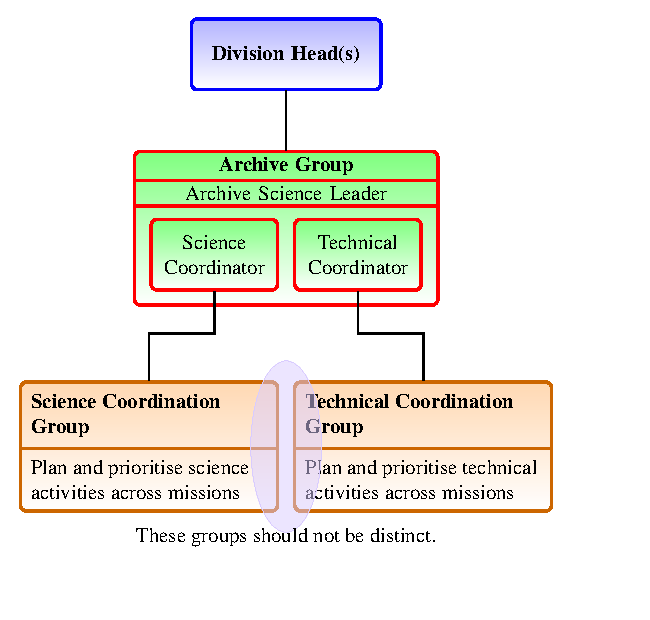
\includegraphics[width=\textwidth]{images/AGcoordinated}
\end{center}
\column{0.4\textwidth}
\begin{itemize}
\item can use onslide to make things appear in order 
\item not done here look up on internet
\end{itemize}
\end{columns}
}


\end{document}
